\documentclass[12pt]{article}
\usepackage[top=1in, bottom=1in, left=1in, right=1in]{geometry}
\usepackage[justification=centering]{caption}
\usepackage{graphicx}
\usepackage{booktabs}
\usepackage{hyperref}
\usepackage{setspace}
\usepackage{cleveref}
\usepackage[per-mode=symbol]{siunitx}
\usepackage{textgreek}
\usepackage[version=3]{mhchem}

\crefformat{footnote}{#2\footnotemark[#1]#3}

\title{The Effects of Diet on Esterase Activity in Bean Beetles}
\author{Samuel Deslandes \and Cynthia Duque \and Roseline Idoko}
\date{\today}
\begin{document}
\maketitle


\doublespacing

\section{Introduction} 
	\textit{Callosobruchus maculatus}, commonly referred to as Bean Beetles, are agricultural pests of Africa and Asia whose larvae feed and develop exclusively on the seed of legumes such as mung beans (\textit{Vigna radiata}) and cowpeas (\textit{Vigna unguiculata}) destroying the crop in the process.\footnote{\label{Handbook}Handbook} In order to combat these pests, organophosphate insecticides such as malaoxon have been used. These insecticides interfere with the insect's nervous system by inhibiting acetylcholinesterase (AChE), an important enzyme in the synaptic transmission process which breaks down the neurotransmitter acetylcholine, thus terminating the signal.\footnote{\label{manual}Manual} By inhibiting AChE signals are never terminated resulting in overestimation and the eventual death of the insect. 
	
	Some insects however, have been documented to be able resist these insecticides. The food source for these insects seem to have an effect on the insect's ability to detoxify the insecticide. Different plants make use of various defensive chemicals to deter their predators. In response to this some insects have evolved mechanisms to detoxify the plant's defenses, one of which being through the detoxification activity of esterase enzymes. This method of resistance may also allow these insects to resist insecticides such as malaoxon, as the esterase enzymes would cleave the esters present in the insecticide, thus rendering it ineffective. It has however not yet been reported this method of detoxification is utilized by the Bean Beetles.\cref{manual} In order to address this, it hypothesized that different food sources will have different effects on the level of activity of esterase enzymes. The null hypothesis is that the food source has no effect on the level of esterase enzyme activity. 
	
\section{Design}
	In order to test this hypothesis crude protein extractions were made from beetles of the species \textit{Callosobruchus maculatus}, reared on two different food sources: mung beans, and cowpeas. All beetles used were of the Mali strain. The crude protein extraction were made following the procedure seen in the lab manual. In order to quantify the level of enzyme activity of each beetle colorimetric enzyme assays were performed as outlined in the lab manual. 
\subsection{Enzyme Assay}
	This enzyme assay uses two specific substrates \textalpha-naphtyl acetate and \textbeta-naphtyl acetate which hydrolyze to produce  \textalpha-naphtyl and \textbeta-naphtyl in the presence of certain esterase enzymes. These products interact with a dye (Fast Blue B Salt), which changes the absorbency of the dye at a specific wavelength.\cref{manual} It is the change in absorbance at this wavelength that is being measured by this assay; A higher change in absorbance corresponds to more enzyme activity, and vice versa.   
\subsection{Protein Assay}
	In order to standardize the amount of protein in each extract a colorimetric protein assay was also performed following the procedure in the lab manual. This assay uses the dye Coomassie brilliant blue G-250 which binds to proteins creating a change in light absorbace by the dye. The measurements from this assay are compared to a standardized curve established using known concentrations of a protein.\cref{manual}
	
	Both assays were performed for each of the substrates \textalpha-naphtyl acetate and \textbeta-naphtyl acetate. Sample sizes vary between treatments and substrates used. (See \cref{refTable}) The entire experiment was performed once. It was predicted that if esterase enzyme activity is measured using change of absorbance of a dye as a proxy for beetles of the same species (\textit{Callosobruchus maculatus}) and strain (Mali), but reared on different food sources, then between each treatment there will be a difference in the absorbency of the dye.
	
	\begin{table}[h]
		\centering
		\begin{tabular}{|l|l|}
			\hline
			Variables:&\\
			\qquad Independent & Food source \\ \hline
			\qquad Dependent & Change of absorbance of \textalpha-naphtyl (\si{AU})\\& Change of absorbance of \textbeta-naphtyl (\si{AU})\\ \hline
			\qquad Standardized & \quad\textbullet\ Beetle species\\ 
			& \quad\textbullet\ Beetle strain \\
			& \quad\textbullet\ Dye \\
			& \quad\textbullet\ Incubation times \\
			& \quad\textbullet\ Amount of substrate added\\ \hline
			Levels of treatment & 2\\
			& \quad\textbullet\ Mung bean \\
			& \quad\textbullet\ Cowpea\\ \hline
			Replications & 1 \\ \hline
			Sample size: &\\
			\qquad \textalpha-naphtyl acetate, Mung bean & 33 \\
			\qquad \textalpha-naphtyl acetate, Cowpea & 32 \\
			\qquad \textbeta-naphtyl acetate, Mung bean & 21 \\
			\qquad \textbeta-naphtyl acetate, Cowpea & 24 \\
			\hline
		\end{tabular}
		\caption{Quick reference table of experiment design}
		\label{refTable}
	\end{table}
	
	The collected data was standardized for protein content and the averages and standard deviations of each level of treatment were calculated. A two-tailed Student's t-test was also performed to ensure statistical significance of the collected data. See the "Results" section below. \newpage
	
\section{Results}
	The standardized curve made from the BSA solutions of known concentration can be seen in figure \ref{stdcurve}. The approximated function of the curve with an r-squared value of 0.986 is:
	\begin{equation}
	F(x)=0.3976\ln x-1.2432
	\end{equation}
	
	\begin{figure}[h]
		\centering
		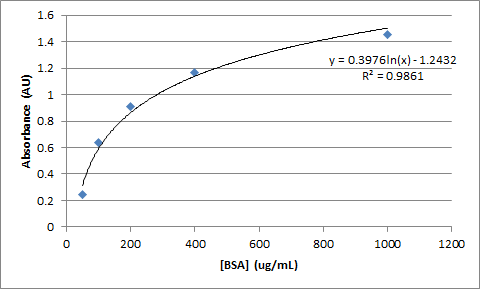
\includegraphics{stdcurve.png}
		\caption{Plot of absorbance (\si{AU}) vs BSA concentration (\si{\micro\gram\per\milli\liter}) for solutions of known concentrations}
		\label{stdcurve}
	\end{figure}
\subsection{Sample calculation}

\section{Discussion}


\subsection{Conclusion}


\section{References}


\end{document}
